\documentclass{beamer}
\usepackage[polish]{babel}
\usepackage[utf8]{inputenc}
\usepackage{lmodern}
\usepackage{polski}
\usepackage{amsfonts}
\usepackage{eufrak}
\usepackage{indentfirst}
\usepackage{amsthm}
\usepackage{multirow}
\usepackage{amsmath}
\usepackage{graphicx}
\newcommand{\norm}[1]{\left\lVert#1\right\rVert}
\usetheme{AGH}

\title{Nierówności wyrocznie dla problemów odwrotnych}
\subtitle{Praca magisterska}
\author{Grzegorz Mika}
\institute{Wydział Matematyki Stosowanej}

\date{5 września 2018}

\begin{document}

\titleframe[pl]


\begin{frame}\frametitle{Początki}\framesubtitle{Matematyczny opis}

\begin{block}{Stochastyczny problem odwrotny}
\begin{displaymath}
Y=Kf+\epsilon\xi
\end{displaymath}
\begin{displaymath}
K\colon \mathbb{H}\to \mathbb{G}, \epsilon>0
\end{displaymath}
\end{block}
\begin{block}{Hubble}
\begin{displaymath}
Y=\int_Dh(\cdot-x)f(x)dx+\epsilon\xi
\end{displaymath}
\begin{displaymath}
\mathbb{H}= \mathbb{G}=L_2(\mathbb{R}^2), h\colon \mathbb{R}^2\to \mathbb{R}
\end{displaymath}
\end{block}
\end{frame}



\begin{frame}\frametitle{Koniec}
\begin{center}
\huge{\textbf{Dziękuję za uwagę!}}
\end{center}
\end{frame}
\begin{frame}\frametitle{Rezultaty}
\begin{center}
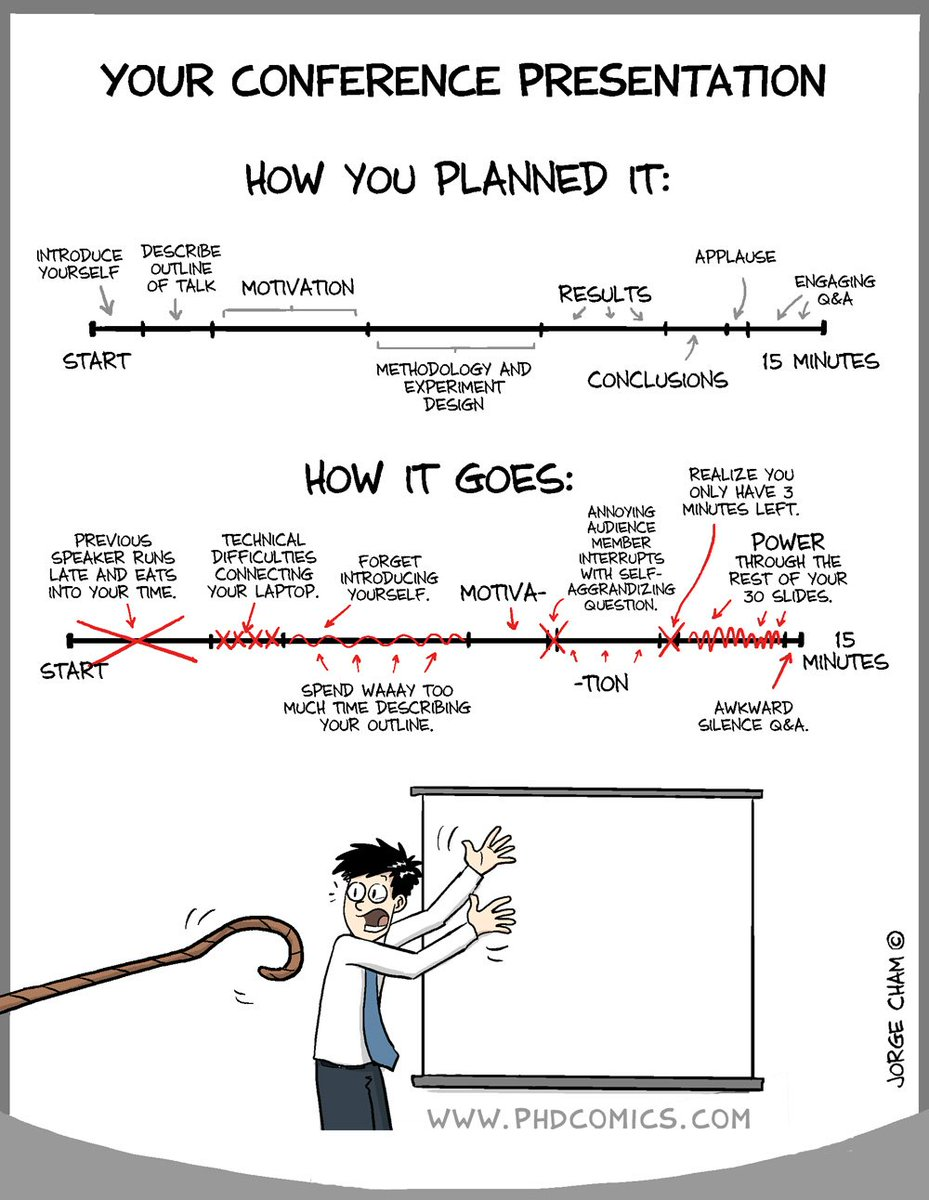
\includegraphics[scale=0.16]{1}
\end{center}
\end{frame}
\end{document}
